%Art des Dokuments%
\documentclass[a4paper, 11pt]{article}

%Packete
\usepackage{ifxetex,ifluatex}
\usepackage{etoolbox}
\usepackage[svgnames]{xcolor}
\usepackage{amssymb}
\usepackage{tikz}
\usepackage{tcolorbox}
\usepackage{framed}

% conditional for xetex or luatex
\newif\ifxetexorluatex
\ifxetex
\xetexorluatextrue
\else
\ifluatex
\xetexorluatextrue
\else
\xetexorluatexfalse
\fi
\fi
%
\ifxetexorluatex
\usepackage{fontspec}
\usepackage{libertine} % or use \setmainfont to choose any font on your system
\newfontfamily\quotefont[Ligatures=TeX]{Linux Libertine O} % selects Libertine as the quote font
\else
\usepackage[utf8]{inputenc}
\usepackage[T1]{fontenc}
\usepackage{libertine} % or any other font package
\newcommand*\quotefont{\fontfamily{LinuxLibertineT-LF}} % selects Libertine as the quote font
\fi

\newcommand*\quotesize{60} % if quote size changes, need a way to make shifts relative
% Make commands for the quotes
\newcommand*{\openquote}
{\tikz[remember picture,overlay,xshift=-4ex,yshift=-2.5ex]
	\node (OQ) {\quotefont\fontsize{\quotesize}{\quotesize}\selectfont``};\kern0pt}

\newcommand*{\closequote}[1]
{\tikz[remember picture,overlay,xshift=4ex,yshift={#1}]
	\node (CQ) {\quotefont\fontsize{\quotesize}{\quotesize}\selectfont''};}

% select a colour for the shading
\colorlet{shadecolor}{Azure}

\newcommand*\shadedauthorformat{\emph} % define format for the author argument

% Now a command to allow left, right and centre alignment of the author
\newcommand*\authoralign[1]{%
	\if#1l
	\def\authorfill{}\def\quotefill{\hfill}
	\else
	\if#1r
	\def\authorfill{\hfill}\def\quotefill{}
	\else
	\if#1c
	\gdef\authorfill{\hfill}\def\quotefill{\hfill}
	\else\typeout{Invalid option}
	\fi
	\fi
	\fi}
% wrap everything in its own environment which takes one argument (author) and one optional argument
% specifying the alignment [l, r or c]
%
\newenvironment{shadequote}[2][l]%
{\authoralign{#1}
	\ifblank{#2}
	{\def\shadequoteauthor{}\def\yshift{-2ex}\def\quotefill{\hfill}}
	{\def\shadequoteauthor{\par\authorfill\shadedauthorformat{#2}}\def\yshift{2ex}}
	\begin{snugshade}\begin{quote}\openquote}
		{\shadequoteauthor\quotefill\closequote{\yshift}\end{quote}\end{snugshade}}


\usepackage[ngerman]{babel}
%\usepackage[latin1]{inputenc}
\usepackage{color}
\usepackage[a4paper, lmargin={4cm}, rmargin={2cm}, tmargin={2,5cm}, bmargin={2,5cm}]{geometry}
\usepackage{graphicx}
\usepackage{setspace}
\usepackage{framed}
\usepackage{url}
\usepackage{eurosym}
\usepackage{acronym}
\usepackage{listings}
\usepackage{color}
\usepackage{longtable}
\usepackage{courier}
\usepackage[multiple]{footmisc}
\usepackage{selinput}
\usepackage{array}
\usepackage{multirow}
\usepackage{longtable}
\usepackage{booktabs}
\usepackage[framemethod=TikZ]{mdframed}
%mdframed Einstellungen%
\newenvironment{theo}[2][]{%
	\refstepcounter{theo}
	
	% Code for box design goes here.
	
	\begin{mdframed}[]\relax}{%
\end{mdframed}}
\ifstrempty{#1}%
% if condition (without title)
{\mdfsetup{%
		frametitle={%
			\tikz[baseline=(current bounding box.east),outer sep=0pt]
			\node[anchor=east,rectangle,fill=blue!20]
			{\strut Definition~\thetheo};}
	}%
	% else condition (with title)
}{\mdfsetup{%
		frametitle={%
			\tikz[baseline=(current bounding box.east),outer sep=0pt]
			\node[anchor=east,rectangle,fill=blue!20]
			{\strut Definition~\thetheo};}%
	}%
}%
% Both conditions
\mdfsetup{%
	innertopmargin=10pt,linecolor=blue!20,%
	linewidth=2pt,topline=true,%
	frametitleaboveskip=\dimexpr-\ht\strutbox\relax%
}
%Umlaute und Kommandos%

\newcommand*{\theadtext}[1]{{\tiny #1}}
\newcommand*{\thead}[1]{\multicolumn1{@{}c@{}}{\theadtext{#1}}}
\newcolumntype{C}[1]{>{\centering\arraybackslash\hspace{0pt}}p{#1}}
\newcolumntype{L}[1]{>{\raggedright\arraybackslash\hspace{0pt}}p{#1}}
\newcolumntype{R}[1]{>{\raggedleft\arraybackslash\hspace{0pt}}p{#1}}
\newcounter{pos}
\newcommand*{\pos}{\refstepcounter{pos}\thepos}
\newcommand{\sectionnumbering}[1]{% 
	\setcounter{section}{0}% 
	\renewcommand{\thesection}{\csname #1\endcsname{section}}} 
\newcommand{\Autor}{Tim Saupp}
\newcommand{\MatrikelNummer}{2742603}
\newcommand{\Kursbezeichnung}{TINF15B3}
\newcommand{\FirmenLogoDeckblatt}{\fbox{
\includegraphics[width=3cm]{dhbw-logo}}}
\newcommand{\Was}{Studienarbeit}
\newcommand{\Titel}{Titel ausstehend}
\newcommand{\AbgabeDatum}{18.09.2017}
\newcommand{\Dauer}{03.07.2017-15.09.2017}
\newcommand{\Abschluss}{Bachelor of Engineering}
\newcommand{\Studiengang}{Informationstechnik}
\newcommand{\BetreuerDHBW}{Prof. Dr. Lausen}

\makeatletter
\newcommand*{\maintoc}{% Hauptinhaltsverzeichnis
	\begingroup
	\@fileswfalse% kein neues Verzeichnis öffnen
	\renewcommand*{\appendixattoc}{% Trennanweisung im Inhaltsverzeichnis
		\value{tocdepth}=-10000 % lokal tocdepth auf sehr kleinen Wert setzen
	}%
	\tableofcontents% Verzeichnis ausgeben
	\endgroup
}
\newcommand*{\appendixtoc}{% Anhangsinhaltsverzeichnis
	\begingroup
	\edef\@alltocdepth{\the\value{tocdepth}}% tocdepth merken
	\setcounter{tocdepth}{-10000}% Keine Verzeichniseinträge
	\renewcommand*{\contentsname}{% Verzeichnisname ändern
		Verzeichnis der Anh\"ange}%
	\renewcommand*{\appendixattoc}{% Trennanweisung im Inhaltsverzeichnis
		\setcounter{tocdepth}{\@alltocdepth}% tocdepth wiederherstellen
	}%
	\tableofcontents% Verzeichnis ausgeben
	\setcounter{tocdepth}{\@alltocdepth}% tocdepth wiederherstellen
	\endgroup
}
\newcommand*{\appendixattoc}{% Trennanweisung im Inhaltsverzeichnis
}
\g@addto@macro\appendix{% \appendix erweitern
	\if@openright\cleardoublepage\else\clearpage\fi% Neue Seite
	\addtocontents{toc}{\protect\appendixattoc}% Trennanweisung in die toc-Datei
}
\makeatother
%Grafische Einstellungen%
\clubpenalty = 100
\widowpenalty = 100
\definecolor{dkgreen}{rgb}{0,0.6,0}
\definecolor{gray}{rgb}{0.5,0.5,0.5}
\definecolor{mauve}{rgb}{0.58,0,0.82}
\definecolor{eggshell}{rgb}{0.94, 0.92, 0.84}
\lstset{
	backgroundcolor=\color{eggshell},
	basicstyle=\footnotesize\ttfamily,
	frame=single,
	breaklines=true,	
	commentstyle=\color{dkgreen},
	captionpos=b,
	keywordstyle=\color{blue},
	stringstyle=\color{mauve},
	tabsize=2,
	language=Java,
	numbers=left,
	numbersep=5pt,
	numberstyle=\tiny\color{gray},
	showstringspaces=false}
%Umbenennung der Zusammenfassung zu Abstract%
\addto\captionsngerman{\renewcommand{\abstractname}{Abstract}}

%%%%%%%%%%%%%%%%%%%%%%%%%%%%%%%%%%%%%%%%%%%%%%%%%%%
%Tim Saupp Studienarbeit 2017-2018 5.& 6. Semester%
%%%%%%%%%%%%%%%%%%%%%%%%%%%%%%%%%%%%%%%%%%%%%%%%%%%
%Anfang des Dokuments%
\begin{document}
\begin{titlepage}
	\begin{center}
		\vspace*{-2cm}
		\FirmenLogoDeckblatt\hfill
\includegraphics[width=5cm]{logo.jpg}\\[2cm]
		{\Huge \Titel}\\[2cm]
		{\Huge\scshape \Was}\\[2cm]
		{\large für die Prüfung zum}\\[0.5cm]
		{\Large \Abschluss}\\[0.5cm]
		{\large des Studienganges \Studiengang}\\[0.5cm]
		{\large an der}\\[0.5cm]
		{\large Dualen Hochschule Baden-Württemberg Karlsruhe}\\[0.5cm]
		{\large von}\\[0.5cm]
		{\large\bfseries \Autor}\\[1cm]
		{\large Abgabedatum \AbgabeDatum}
		\vfill
	\end{center}
	\begin{tabular}{l@{\hspace{2cm}}l}
		Bearbeitungszeitraum	         & \Dauer 			\\
		Matrikelnummer	                 & \MatrikelNummer		\\
		Kurs			         & \Kursbezeichnung		\\
		Gutachter der Studienakademie	 & \BetreuerDHBW		\\
	\end{tabular}
\end{titlepage}
\newpage
\thispagestyle{empty}
\begin{framed}
	\begin{center}
		\Large\bfseries Erklärung
	\end{center}
	\medskip
	\noindent
	Ich versichere hiermit, dass ich meine \Was\ mit
	dem Titel: {\Titel} selbstständig verfasst und keine anderen als die angegebenen Quellen und
	Hilfsmittel benutzt habe. Ich versichere zudem, dass die eingereichte elektronische Fassung mit der
	gedruckten Fassung übereinstimmt.
	
	\vspace{3cm}
	\noindent
	\underline{\hspace{4cm}}\hfill\underline{\hspace{6cm}}\\
	Ort~~~~~Datum\hfill Unterschrift\hspace{4cm}
\end{framed}
\newpage
\begin{framed}
	\begin{center}
		\Large\bfseries Sperrvermerk
	\end{center}
	\medskip
	\noindent
	Der Inhalt dieser Arbeit darf weder als Ganzes noch in Auszügen Personen
	außerhalb des Prüfungsprozesses und des Evaluationsverfahrens zugänglich gemacht
	werden, sofern keine anders lautende Genehmigung der Ausbildungsstätte vorliegt.
\end{framed}
\newpage
\pagenumbering{Roman} 
\begin{abstract}
Hier Abstract.
\end{abstract}
\newpage
\maintoc           % Inhaltsverzeichnis hier ausgeben%
\newpage
\listoffigures             % Liste der Abbildungen%
\newpage
\listoftables              % Liste der Tabellen%
\newpage
\section*{\Large \textbf Abkürzungsverzeichnis}  
\begin{acronym}[Bash]
	\acro{DUM}{DUMMY}
\end{acronym}
\newpage
\pagenumbering{arabic} 
\section{Projektbeschreibung}
\subsection{Motivation}
\subsection{Ziel der Arbeit}
\subsection{Kapitelübersicht}
\newpage
\section{Grundlagen}
\subsection{Schwarmintelligente Superorganismen}
\subsubsection{Begriffsdefintion}
Bereits 1911 bezeichnet W. M. Wheeler, amerikanischer Ethologe mit Spezialisierung auf dem Gebiet der Erforschung sozialer Insekten, Kolonien wie die der Bienen und Ameisen als \textit{Superorganismen mit emergenten Fähigkeiten}\footnote{W.M. Wheeler (1911)}.\newline
\par Durch die sensuale Verbindung der Tiere wird die Futtersuche/-versorgung und das Abwehren von Gefahren ohne eine zentrale Lenkung bzw. ohne hierarchische Befehlskette bewältigt. Instinktiv verankerte Regeln sorgen dafür, dass auf bestimmte Aktionen der Tiere in vollkommen deterministischer Weise eine Reaktion erfolgt. Aus dieser dezentralen Interaktion entstehen, bei einem Kollektiv von Tieren, intelligente Resultate auf Makroebene.
\newline\newline\newline
Andreas Aulinger beschreibt die Entstehungsbedingungen und Definitionen kollektiver Intelligenz bei Tierschwärmen wie folgt\footnote{A. Aulinger (2013)}:\newline
\begin{figure}[h]
	\begin{center}
	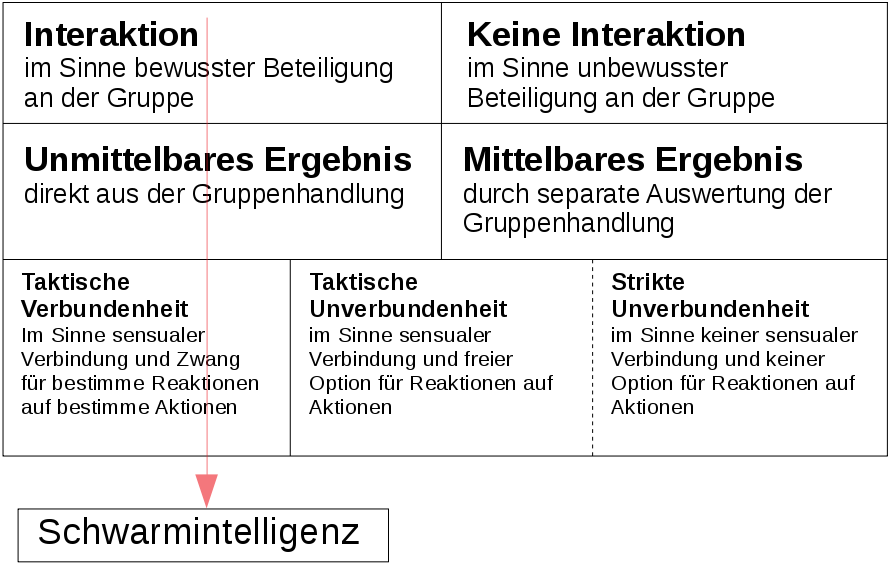
\includegraphics[width=1\textwidth]{schwarmintelligenz}
	\end{center}
	\hspace{1in}\parbox{4in}{\caption{Entstehungsbedingungen und Definitionen kollektiver Intelligenz bei Tierschwärmen}}
\end{figure}
\begin{itemize}
	\item \textbf{Interaktion:} Auf Aktion und Reaktion basierende Interaktion gilt als Grundlage bzw. Rahmenbedingung für die Definition des Begriffs Schwarmintelligenz. Anlass dafür ist der in den Tieren vorhandene Instinkt, der diese veranlasst, sich bewusst an der Gruppe zu beteiligen.
	\item \textbf{Unmittelbares Ergebnis:} Einzelne Tiere führen Handlungen aus ohne Wissen um das Schwarmergebnis. Das Resultat entsteht unmittelbar aus der Handlung des Schwarms und bedarf keiner externen Aggregation und Auswertung.
	\item \textbf{Taktische Verbundenheit:} Sowohl die sensuale Verbindung der Tiere als auch der in den Tieren verankerte Instinkt zeugen von der taktischen Verbundenheit des Schwarms bestehend aus festen Aktions- und Reaktionsmustern. 
\end{itemize}
\par Zusammenfassend beschreibt der Begriff Schwarmintelligenz ein Phänomen aus dem Tierreich zur Selbstorganisation eines Schwarms um lebensnotwendige Aufgaben gemeinsam und auf intelligente Weise zu bewältigen. Dabei vollbringen die Tiere im Schwarm Leistungen, die das Vermögen jedes Einzeltiers übersteigen.
\subsubsection{Ameisen}
Eine einzelne Ameise ist nicht überlebensfähig. Im Gegensatz dazu vollbringt ein Ameisenstaat Erstaunliches und passt sich an neue Gegebenheiten seiner Umwelt an. Ameisen bilden Staaten mit einigen hundert bis zu mehreren Millionen Individuen. Trotz dieser riesigen Anzahl funktioniert ein Ameisenstaat, da er sich selbst organisiert ohne eine hierarchische Instanz, die einen Überblick über alle Aufgaben besitzt oder diese steuert und verteilt. Stattdessen führen die Handlungen einzelner Ameisen im Zusammenspiel zu einem organisierten Staat, der für die Ameisen sorgt und Nahrung, Brutpflege und Schutz zur Verfügung stellt. Für die Informatik besonders interessant sind die Ameisen aufgrund ihrer Fähigkeit effiziente Wege zwischen Futterquellen und dem Ameisenbau ausfindig zu machen\footnote{L. Pintscher (2008)}.
\par Ist der Futtervorrat des Ameisenbaus erschöpft verlassen mehrere Ameisen den Ameisenbau gleichzeitig und begeben sich auf Futtersuche. Sobald die Ameise eine Futterquelle gefunden hat, nimmt sie eine Gewichtseinheit des Futters mit und begibt sich auf den Rückweg zum Ameisenbau. Dabei setzt die Ameise Pheromone frei die mit der Zeit verfliegen, um den Weg zur Futterquelle zu markieren. Die Ameise die den kürzesten Weg zu einer Futterquelle gefunden hat legt die Strecke zwischen Ameisenbau und Futterquelle häufiger zurück.  Die Pheromonspur wird durch das häufige Zurücklegen der Strecke intensiviert und dient als sicherer Wegweiser zur Futterquelle. Mitglieder der Kolonie folgen den intensivsten Pheromonspuren. Ist die Futterquelle erschöpft, löst sich die Pheromonspur auf\footnote{R. Wehner (2001)}.
\subsubsection{Bienen}
Um den Gesamtenergiebedarf des Schwarms zu ermitteln, orientiert sich die einzelne Sammlerin an der Wartezeit bei der Übergabe des gesammelten Nektars an die Bienen die den Nektar speichern: Je voller die Futterspeicher, desto länger müssen die Speicherbienen nach leeren Zellen suchen. Je leerer die Speicher, desto schneller wird die Abgabe des Nektars abgewickelt\footnote{A. Aulinger (2013)}.
\par Im kilometerweiten Gelände besitzt keine Biene den gesamten geographischen Überblick. Sie entscheidet nur lokal über die Rentabilität der Futterquelle. Kundschafterinnen und Sammlerinnen, die von der Futtersuche wiederkehren, führen einen Tanz auf und zeigen unbeschäftigten Bienen damit die Richtung und Entfernung  Futterquelle. Unbeschäftigte Bienen sehen sich die Tänze ankommender Bienen an und entscheiden sich anschließend für ihr nächstes Ziel. Sobald eine Futterquelle erschöpft ist brauchen die Sammlerinnen länger beim Sammeln und veranlassen aufgrund der geringeren Anzahl an Tänzen weniger Bienen dazu am gleichen Ort zu sammeln.
\subsection{Agentenbasierte Modellierung}
Die Agentenbasierte Modellierung erlaubt eine natürliche Beschreibung von Systemen als eine Sammlung autonomer entscheidungsfähiger Agenten, um emergente Phänomene zu analysieren. Das Ziel der Agentenbasierten Modellierung besteht darin, durch die Simulation einer Vielzahl an Agenten, das resultierende Systemverhalten zu untersuchen. 
\newline\newline\newline
Nach Macal und North, verfügt ein agentenbasiertes System über drei Komponenten:
\begin{itemize}
	\item \textbf{Agenten:} Agenten handeln auf der Basis von festgelegten Regeln.
	\item \textbf{Agenten-Beziehungen:} Beziehungen zwischen Agenten entstehen durch proaktive Aktion eines Agenten und die darauffolgende Reaktion eines anderen Agenten.
	\item \textbf{Agenten-Umgebung:} Sämtliche Agenten werden innerhalb einer Umgebung modelliert.
\end{itemize}
\par Wooldridge und Jennings weisen Agenten die Charaktereigenschaften Autonomie, Interaktivität, Reaktivität und Proaktivität zu. 
\subsection{Schwarmintelligente Algorithmen}
\subsubsection{Particle Swarm Optimization}
\subsubsection{Ant Colony Optimization}
\subsubsection{Bee Colony Optimization}
\newpage
\begin{thebibliography}{sotief}
	\bibitem{1}W.M. Wheeler. The Ant Colony as an Organism. Journal of Morphology Volume 22, Issue 2, Seite 307-325. Weblink:
	http://www3.interscience.wiley.com/journal/109914213/abstract. EJ: 1911. Einsichtnahme: 25.02.2018
\end{thebibliography}
\newpage
\appendix
\appendixtoc
\newpage
\section{Anhang 1} 
\end{document}


